\documentclass[11pt]{article}
\usepackage[utf8]{inputenc}
\usepackage[T1]{fontenc}
\usepackage{babel}
\usepackage[top=2.5cm, bottom=2.5cm, left=2.5cm, right=2.5cm]{geometry}
\usepackage{xcolor}
\usepackage{hyperref}
\usepackage{titlesec}
\usepackage{enumitem}
\usepackage{mdframed}
\usepackage{fancyhdr}
\usepackage{graphicx}

% Couleurs
\definecolor{violetuniv}{RGB}{100, 50, 150}
\definecolor{rougetitre}{RGB}{200, 50, 50}
\definecolor{borduregrise}{RGB}{180, 180, 180}

% Liens hypertexte
\hypersetup{
    colorlinks=true,
    linkcolor=violetuniv,
    urlcolor=violetuniv,
}

% Style des titres de section
\titleformat{\section}{\large\bfseries}{}{0em}{}
\titleformat{\subsection}{\normalsize\bfseries}{}{0em}{}

% En-tête
\pagestyle{fancy}
\fancyhf{}
\renewcommand{\headrulewidth}{0.4pt}
\fancyhead[L]{\small\textcolor{violetuniv}{Conception Web -- Semestre 2}}
\fancyfoot[C]{\thepage}

% Environnement "À faire"
\newmdenv[
    linecolor=borduregrise,
    backgroundcolor=white,
    linewidth=1pt,
    leftmargin=0pt,
    rightmargin=0pt,
    innerleftmargin=10pt,
    innerrightmargin=10pt,
    innertopmargin=8pt,
    innerbottommargin=8pt,
]{afaire}

\begin{document}

\thispagestyle{empty}
\vspace*{3cm}

\begin{center}
    {\small\textcolor{violetuniv}{Université d'Avignon -- CERI}}\\[0.5cm]
    {\small\textcolor{violetuniv}{Licence Informatique -- Semestre 2}}\\[2cm]

    {\rule{\linewidth}{0.5pt}}\\[0.4cm]
    {\LARGE\bfseries Conception Web}\\[0.3cm]
    {\large TP0 -- (Optionnel) Internet, le Web et HTML}\\[0.4cm]
    {\rule{\linewidth}{0.5pt}}\\[2cm]

    {\large Module : S-E06-0158}\\[0.5cm]
    {\large Année universitaire 2025--2026}\\[3cm]

    \begin{tabular}{ll}
        \textbf{Enseignant :} & Fabrice LEFEVRE -- CERI \\
        \textbf{Niveau :}     & Licence 1 Informatique \\
        \textbf{Semestre :}   & Semestre 2 \\
    \end{tabular}
\end{center}

\vfill

\begin{center}
    \textcolor{borduregrise}{\rule{\linewidth}{0.3pt}}\\[0.3cm]
    {\small\textit{Ce document regroupe les sujets des TP 0.1 à 0.5 du module Conception Web.}}
\end{center}
% ============================================================
\newpage
\fancyhead[R]{\small TP 0.1 -- Utilisation d'un navigateur Web}

{\Large\bfseries TP 0.1 -- Utilisation d'un navigateur Web}

\bigskip

Il existe de nombreux navigateurs Web utilisables gratuitement :

\begin{itemize}
    \item Google Chrome
    \item Edge (sur Windows uniquement)
    \item Mozilla Firefox
    \item Safari
    \item Opera
\end{itemize}

Ils offrent tous sensiblement les mêmes fonctionnalités comme les marques pages (pour la gestion des favoris), le chiffrement de contenu (pour les échanges sécurisés) ou les fenêtres multi-onglets (pour une navigation rapide en passant d'une page à l'autre facilement).

\section{Rappel sur les URL}

Une URL permet de désigner l'emplacement d'une ressource sur le Web (voir la diapositive 34 du cours pour plus de détails).

\begin{afaire}
\textbf{À faire :}

Ouvrez les pages suivantes et constatez les différences (copier-coller les liens pour aller plus vite) :

\begin{itemize}
    \item \url{http://www.univ-avignon.fr}
    \item \url{https://www.mozilla.org/fr/}
    \item \url{https://doc.ubuntu-fr.org/}
    \item \texttt{ftp://ftp.fr.debian.org/debian/}
    \item \texttt{file:///}
\end{itemize}
\end{afaire}

Les navigateurs web sont capables d'accéder aux ressources d'une multitude de manières, y compris celles stockées sur votre machine. On pourra donc réaliser des pages Web ou des sites entiers sans avoir à les publier sur Internet.

\section{Les outils de développement}

Les navigateurs modernes incluent des outils pour aider les développeurs à créer des pages Web. Le plus intéressant est l'inspecteur de code, il permet de visualiser la structure d'une page HTML et d'examiner les propriétés de chaque élément comme sa position, sa taille et même les règles CSS qui y sont appliquées (nous y reviendrons plus tard dans le semestre).

Pour ouvrir l'inspecteur de code :

\begin{itemize}
    \item Avec Firefox : dans le menu ``Développement'' puis ``Inspecteur'' ou via le raccourci \texttt{Ctrl + Maj + C}.
    \item Avec Google Chrome : dans le menu ``Outils'' puis ``Outils de développement'' ou via le raccourci \texttt{Ctrl + Maj + I} ou \texttt{F12}.
\end{itemize}

\begin{afaire}
\textbf{À faire :}

Ouvrir la page sur le World Wide Web de Wikipedia (\url{https://fr.wikipedia.org/wiki/World_Wide_Web}) et explorer la structure de cette dernière.

Retrouver les éléments suivants :

\begin{itemize}
    \item Le titre principal ``World Wide Web'' : balise \texttt{<h1>}
    \begin{itemize}
        \item Remplacer ce titre par ``World Wide Web (WWW)'' dans l'inspecteur de code (puis vérifier que cette modification s'affiche immédiatement mais ne reste pas si vous rechargez la page)
    \end{itemize}
    \item L'image du logo du World Wide Web (à droite) : balise \texttt{<img>}
    \item Sauvegarder la page sur votre disque dur local (depuis le menu Fichier)
    \item Fermer l'onglet puis :
    \begin{itemize}
        \item Ouvrir la page en utilisant l'URL
        \item Ouvrir dans un deuxième onglet la page sauvegardée localement
        \item Constater que le titre n'a pas été modifié sur la page utilisant l'URL mais qu'il est modifié sur celle enregistrée sur votre disque dur
    \end{itemize}
\end{itemize}
\end{afaire}

En cas de mauvais affichage ou d'un résultat inattendu, l'inspecteur de code peut aider à cerner les problèmes les plus courants (balises mal imbriquées, balise fermante manquante, faute de frappe, etc.). Durant les TP n'hésitez pas à abuser de cet outil pour vous aider à résoudre les problèmes.

\vspace{1em}
\noindent\textit{Last modified: Sunday, 8 March 2026, 6:29 PM}

% ============================================================
\newpage
\fancyhead[R]{\small TP 0.2 -- Savoir où trouver l'information}

{\Large\bfseries TP 0.2 -- Savoir où trouver l'information}

\bigskip

Le Web regorge de ressources concernant le HTML et le CSS, allant de la documentation officielle à des exemples d'utilisation.

\textbf{Attention toutefois à ne pas utiliser n'importe quoi !}

Le HTML évolue et les navigateurs aussi, certains sites donnent des informations et présentent des techniques qui peuvent être difficiles à comprendre ou à mettre en place.

De même, ne pas copier-coller directement du code dans vos TP (qui n'est pas fourni dans les exercices) car en plus de ne pas vous aider dans votre apprentissage, ils pourraient avoir des effets indirects indésirables.

\section{La recommandation officielle du HTML}

Le HTML et le CSS sont des langages qui offrent énormément de possibilités (il n'y a qu'à voir la multitude de sites Web différents qui existent) et il est parfois difficile de se souvenir des différentes valeurs d'un attribut ou d'une propriété.

\begin{afaire}
\textbf{À faire :}

\begin{itemize}
    \item Retrouver la recommandation officielle du HTML5 datant du 28 octobre 2014 sur le site du W3C (\url{http://www.w3.org}).
    \item Vérifier que la partie 4 ``The elements of HTML'' contient les informations utiles pour la réalisation des futurs TP.
\end{itemize}
\end{afaire}

\section{Une documentation plus lisible}

La documentation officielle bien que complète peut être difficile à lire, même avec un bon niveau d'anglais. Le site W3Schools (\url{http://www.w3schools.com}) présente de manière plus intelligible une référence pour le HTML mais aussi le CSS (ce qui vous sera utile lorsque nous en viendrons à styliser nos pages plus tard dans le module).

Si vous avez du mal avec l'anglais vous pouvez utiliser l'icône monde dans le menu en haut à droite pour traduire le site en français.

\textbf{Attention} : il s'agit d'une traduction automatique, elle peut donc être imprécise.

\newpage
\begin{afaire}
\textbf{À faire :}

Se rendre sur le site W3Schools et à l'aide de la partie ``HTML References'', répondre aux questions suivantes :

\begin{itemize}
    \item Quelle balise permet d'afficher une image ?
    \begin{itemize}
        \item Quel attribut permet de spécifier du texte alternatif à une image ?
    \end{itemize}
    \item Où se situe le doctype ?
    \begin{itemize}
        \item Donner les doctypes du HTML5 ainsi que celui du HTML4 permettant d'utiliser les cadres (frame)
    \end{itemize}
    \item Retrouver la balise permettant de définir un hyperlien
    \begin{itemize}
        \item Quelles sont les différents relations que l'on peut exprimer entre la page incluant le lien et la page sur laquelle mène ce lien (aide : c'est un attribut qui permet de le faire)
    \end{itemize}
\end{itemize}

Les meta-informations sont aussi très importantes, elles donnent des indications sur la page.

\begin{itemize}
    \item Où place-t-on les balises de meta-information \texttt{<meta>} ?
    \item Il est très important de toujours donner l'encodage des caractères utilisés par votre page Web (le navigateur ne peut pas toujours le deviner seul), quel attribut faut-il utiliser ?
    \item Comment donne-t-on un titre à une page Web ?
\end{itemize}
\end{afaire}

\textbf{Astuce :} c'est une bonne idée de mettre en marque page le site du W3Schools afin de pouvoir retrouver les informations plus rapidement pour les prochains TP.

\vspace{1em}
\noindent\textit{Last modified: Sunday, 8 March 2026, 6:30 PM}

% ============================================================
\newpage
\fancyhead[R]{\small TP 0.3 -- Edition de texte}

{\Large\bfseries TP 0.3 -- Edition de texte}

\bigskip

\section{Edition de texte}

\begin{afaire}
\textbf{A faire :}

\begin{enumerate}
    \item Démarrer le bloc-note ou gedit (ou Notepad++ que vous pouvez installer sur votre compte personnel).
    \item Ouvrir la page HTML \url{http://www.w3.org/community/webed/wiki/HTML/Training} avec le navigateur web, l'enregistrer localement (\ldots c'est à dire sur votre disque dur, avec ``\textit{Enregistrer sous\ldots}'').
    \item Modifier son contenu :
    \begin{itemize}
        \item Dupliquer quelques parties des sections ``Week\_2'' ou ``See\_also'' en utilisant le copier-coller.\\
        Aide : ces sections sont identifiées par un \textit{id=}
        \item Localiser le sommaire (\textit{table of contents, toc}) et modifier la définition html du premier niveau de liste pour qu'il soit numéroté automatiquement\\
        Aide : cette partie est balisée par\\
        \texttt{<div id="toc">\ldots</div>}
        \item Essayer d'apporter d'autres modifications\ldots
    \end{itemize}
    \item Enregistrer le fichier avec les modifications. Ouvrir à nouveau dans le navigateur. Vérifier que les modifications sont bien visibles.
\end{enumerate}
\end{afaire}

\newpage
\section{Votre premier fichier HTML}

\begin{afaire}
\textbf{A faire :}

\begin{enumerate}
    \item Créer un nouveau fichier dans l'éditeur de texte.
    \item Récupérer et ouvrir une ossature (squelette) dans les documentations du module. Puis utiliser un copier-coller pour l'insérer dans votre fichier.
    \item Sauvegarder sous le nom ``\texttt{premierepage.html}''.
    \item Donner le nom ``Atelier HTML - Premier Essai'' à votre page web.
    \item Insérer des méta-balises permettant de donner:
    \begin{itemize}
        \item Des informations sur l'auteur de la page :
        \begin{itemize}
            \item nom de l'auteur (ex \textit{Groupe TD1}),
            \item son adresse électronique (ex \textit{l1-ceri@listes.univ-avignon.fr})
        \end{itemize}
        \item Des informations sur la page web :
        \begin{itemize}
            \item sa description (Exemple d'utilisation des balises méta et attributs en HTML),
            \item ses mots-clés (atelier, html),
            \item son Type MIME (text/html), son code ASCII (charset=utf-8) et
            \item son langage (fr).
        \end{itemize}
    \end{itemize}
    Remarque : Voir Partie 2 du cours -- Principes du HTML -- pour toute information concernant les méta-balises.
    \item Insérer ce texte :

    \bigskip
    {\LARGE\bfseries Titre de premier niveau}

    {\Large\bfseries Titre de deuxième niveau}

    Première ligne du paragraphe.\\
    Seconde ligne du paragraphe.

    Le HTML5 est encore un langage \textbf{d'avenir}.

    \item Afficher les informations relatives à la page web créée
    (voir annexe \ref{annexe:infospage}, page \pageref{annexe:infospage}).
    \item Ouvrir le fichier dans le navigateur en le lisant à partir du disque dur.
    \item Faire afficher par le navigateur le source du document web. Vérifier qu'il s'agit bien de votre fichier texte HTML initial.
    \item Tester quelques balises supplémentaires de mise en forme du texte (voir dans le cours).
\end{enumerate}
\end{afaire}

\vspace{1em}
\noindent\textit{Last modified: Friday, 21 September 2018, 10:55 AM}

% ============================================================
\newpage
\fancyhead[R]{\small TP 0.4 -- Premiers pas en HTML}

{\Large\bfseries TP 0.4 -- Premiers pas en HTML}

\bigskip

\section{Bases du HTML}

\subsection{Première page}

Il est demandé de créer une première page HTML de base, à l'aide d'un éditeur de texte standard (BlocNote, WordPad, Notepad++ sous Windows, ou gedit sous Linux par exemple).

\textcolor{rougetitre}{\textbf{Aide :}} Pour vous aider des squelettes (ou ossatures, ie fichiers qui ne contiennent que les déclarations standards du HTML) sont disponibles dans le dernier bloc du module (après les exemples de lien). Vous pouvez en faire une version personnelle (en mettant à jour quelques éléments comme l'auteur\ldots) et ensuite faire un copier-coller de ce fichier pour initialiser chaque exercice.

\textcolor{rougetitre}{\textbf{Attention :}} Penser à respecter les consignes pour les rendus de TP : nom du fichier archive remis sur le Dépôt de travail et contenu de l'archive (copie du sujet de TP et insertion de liens vers les fichiers réponses). Pour ceux qui ne savent pas encore faire de liens HTML vous pourrez attendre le TP prochain avant de mettre cela en application !

\newpage
\subsection{A faire :}

\begin{afaire}
Cette page devra comporter :
\begin{itemize}
    \item un titre dans l'onglet du navigateur
    \item trois paragraphes alignés dans l'ordre : à gauche, à droite et justifié.
    \item des commentaires dans le fichier source (i.e. du texte qui n'apparaît pas dans le navigateur)
\end{itemize}
\end{afaire}

\section{Validation de la page HTML}

Après avoir écrit votre page HTML, vous allez la valider dans un premier temps en la lisant simplement à l'aide d'un navigateur Web. Il sera alors possible de voir apparaître vos erreurs éventuelles :

\begin{itemize}
    \item affichage incorrect : l'affichage ne correspond pas à vos attentes
    \item absence d'affichage : lorsque le navigateur détecte des parties de HTML incorrectes ou trop ambiguës, il choisit de ne pas les afficher du tout
\end{itemize}

Une relecture attentive de la page HTML suffit bien souvent à corriger les erreurs. Il est aussi possible d'utiliser le ``validateur'' de HTML fourni par le W3C. Il vous permettra aussi de détecter des ``erreurs'' HTML que votre navigateur corrige automatiquement (par exemple l'oubli d'une balise fermante dans certains cas), mais aussi les ``erreurs'' dues aux variations entre les différentes versions du langage.

\begin{afaire}
\textbf{A faire :}

\begin{itemize}
    \item Placer une déclaration de type de document (DTD) dans le prologue (\textit{Header}) du document HTML ; tester le résultat de la validation du document sur le site du validateur HTML du W3C (\url{http://validator.w3.org/file-upload.html}), en spécifiant tout d'abord les DTD du HTML 3.2, puis du 4.01 Transitional, et enfin du 5.
\end{itemize}
\end{afaire}

\textcolor{rougetitre}{\textbf{Attention :}} penser aussi à régler le codage (\texttt{encoding} ou \texttt{charset}) correctement

\textcolor{rougetitre}{\textbf{Aide :}} un exemple de déclaration complète de la DTD et du jeux de caractère est donné dans la partie 2 du cours (p. 40).

\vspace{1em}
\noindent\textit{Last modified: Sunday, 8 March 2026, 6:31 PM}

% ============================================================
\newpage
\fancyhead[R]{\small TP 0.5 -- Mise en forme de texte}

{\Large\bfseries TP 0.5 -- Mise en forme de texte}

\bigskip

\section{Mise en forme de texte}

Dans un seul fichier HTML regrouper l'ensemble des exemples demandés ci-dessous pour passer en revue quelques balises de mise en forme du texte.

\textcolor{rougetitre}{\textbf{Attention}} : pour ce TP il faut essayer de ne pas encore utiliser de CSS. Utiliser les ``anciennes'' balises de mise en forme de texte et laisser ensuite le validateur indiquer que vos choix sont obsolètes.

\subsection{A faire :}

\begin{afaire}
\begin{enumerate}
    \item Mettre en forme l'article disponible dans le fichier \texttt{tp1.txt} (accessible sous ce sujet).
    \begin{itemize}
        \item Copier le contenu de l'article dans votre fichier
        \item Appliquer un style de titre au titre général
        \item Ajouter un titre de niveau moindre avant chaque paragraphe
        \item Créer les paragraphes avec des balises \texttt{<p>}
        \item Mettre chaque nom de continent ou de pays en police \texttt{Helvetica} et en bleu
        \item Mettre chaque nom de ville en gras-souligné et en jaune
        \item Placer une barre horizontale d'épaisseur 3 entre chaque paragraphe
        \item Ajouter à la fin du document, après la dernière barre, la date courante (en version statique, i.e. sans utiliser de Javascript !), dans un paragraphe centré
    \end{itemize}
    \item Tester le résultat avec le validateur du W3C
\end{enumerate}
\end{afaire}

\vspace{1em}
\noindent\textit{Last modified: Sunday, 8 March 2026, 6:31 PM}

% ============================================================
% ANNEXES
% ============================================================
\newpage
\fancyhead[R]{\small Annexes}
\appendix

\section{Exemple de résultat -- TP 0.3}
\label{annexe:infospage}

La capture ci-dessous illustre l'affichage des informations relatives à une page web créée lors du TP 0.3 (fenêtre ``Informations sur la page'' de Firefox), montrant les méta-balises correctement renseignées.

\bigskip

\begin{center}
    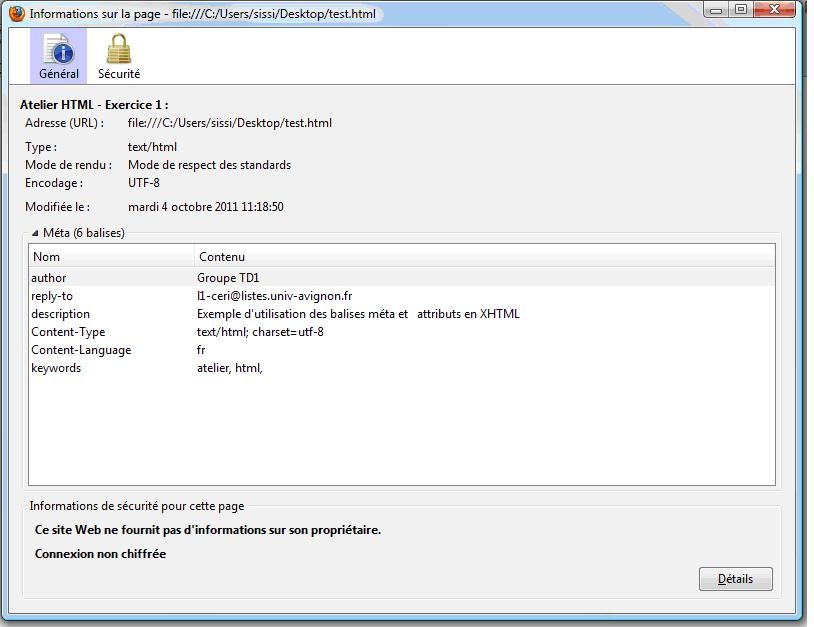
\includegraphics[width=0.75\textwidth]{TP_0.3-photo}
\end{center}

\end{document}